\documentclass[12pt,a4paper]{article}
\usepackage[utf8]{inputenc}
\usepackage[english]{babel}

\usepackage{amsmath}
\usepackage{amsfonts}
\usepackage{amssymb}

\usepackage{graphicx}
\usepackage{lmodern}
\usepackage{tikz}
\usepackage{titlesec}
\usepackage{environ}
\usepackage{xcolor}
\usepackage{fancyhdr}
\usepackage[colorlinks = true, linkcolor = black]{hyperref}
\usepackage{xparse}
\usepackage{enumerate}

\usepackage[left=2cm,right=2cm,top=2cm,bottom=2cm]{geometry}
\usepackage{multicol}

\newcommand{\spaceP}{\vspace*{0.5cm}}
\newcommand{\Span}{\mathrm{Span}\,}

%% Redefining sections
\newcommand{\sectionformat}[1]{%
    \begin{tikzpicture}[baseline=(title.base)]
        \node[rectangle, draw] (title) {#1};
    \end{tikzpicture}
    
    \noindent\hrulefill
}

% default values copied from titlesec documentation page 23
% parameters of \titleformat command are explained on page 4
\titleformat%
    {\section}% <command> is the sectioning command to be redefined, i. e., \part, \chapter, \section, \subsection, \subsubsection, \paragraph or \subparagraph.
    {\normalfont\large\scshape}% <format>
    {}% <label> the number
    {0em}% <sep> length. horizontal separation between label and title body
    {\centering\sectionformat}% code preceding the title body  (title body is taken as argument)

%% Set counters for sections to none
\setcounter{secnumdepth}{0}

%% Set the footer/headers
\pagestyle{fancy}
\fancyhf{}
\renewcommand{\headrulewidth}{0pt}
\renewcommand{\footrulewidth}{2pt}
\lfoot{P.-O. Paris{\'e}}
\cfoot{MATH 307}
\rfoot{Page \thepage}

%% Defining example environment
\newcounter{example}[section]
\NewEnviron{example}%
	{%
	\noindent\refstepcounter{example}\fcolorbox{gray!40}{gray!40}{\textsc{\textcolor{red}{Example~\theexample.}}}%
	%\fcolorbox{black}{white}%
		{  %\parbox{0.95\textwidth}%
			{
			\BODY
			}%
		}%
	}

% Theorem environment
\NewEnviron{theorem}%
	{%
	\noindent\refstepcounter{example}\fcolorbox{gray!40}{gray!40}{\textsc{\textcolor{blue}{Theorem~\theexample.}}}%
	%\fcolorbox{black}{white}%
		{  %\parbox{0.95\textwidth}%
			{
			\BODY
			}%
		}%
	}

%% Commands for matrix of dimensions m x n
%\newcommand{\matMN}[1]{%
%	\begin{bmatrix}
%	#1_{11} & #1_{12} & #1_{13} & \cdots & #1_{1n} \\
%	#1_{21} & #1_{22} & #1_{23} & \cdots & #1_{2n} \\
%	#1_{31} & #1_{32} & #1_{33} & \cdots & #1_{3n} \\
%	\vdots & \vdots & \vdots & \ddots & \vdots \\
%	#1_{m1} & #1_{m2} & #1_{m3} & \cdots & #1_{mn}
%	\end{bmatrix}		
%	}
	
\NewDocumentCommand{\matMN}{mg}{%
	\IfNoValueTF{#2}
		{%
		  \begin{bmatrix}
		   #1_{11} & #1_{12} & #1_{13} & \cdots & #1_{1n} \\
	       #1_{21} & #1_{22} & #1_{23} & \cdots & #1_{2n} \\
		   #1_{31} & #1_{32} & #1_{33} & \cdots & #1_{3n} \\
		   \vdots & \vdots & \vdots & \ddots & \vdots \\
		   #1_{m1} & #1_{m2} & #1_{m3} & \cdots & #1_{mn}
		   \end{bmatrix}	%
		}
		{%
		   \begin{bmatrix}
		   #1_{11} + #2_{11} & #1_{12} + #2_{12} & \cdots & #1_{1n} + #2_{2n} \\
		   #1_{21} + #2_{21} & #1_{22} + #2_{22} & \cdots & #1_{2n} + #2_{2n} \\
		   \vdots & \vdots & \vdots & \ddots & \vdots \\
		   #1_{m1} + #2_{m1} & #1_{m2} + #2_{m2} & \cdots & #1_{mn} + #2_{mn}
		   \end{bmatrix}
		}%
}

%%%%
\begin{document}
\thispagestyle{empty}

\begin{center}
\vspace*{2.5cm}

{\Huge \textsc{Math 307}}

\vspace*{2cm}

{\LARGE \textsc{Chapter 1}} 

\vspace*{0.75cm}

\noindent\textsc{Section 1.1: Systems of Linear Equations}

\vspace*{0.75cm}

\tableofcontents

\vfill

\noindent \textsc{Created by: Pierre-Olivier Paris{\'e}} \\
\textsc{Summer 2022}
\end{center}

\newpage

\section{Why do we care about Systems of Linear Equations?}

\begin{minipage}{0.6\textwidth}
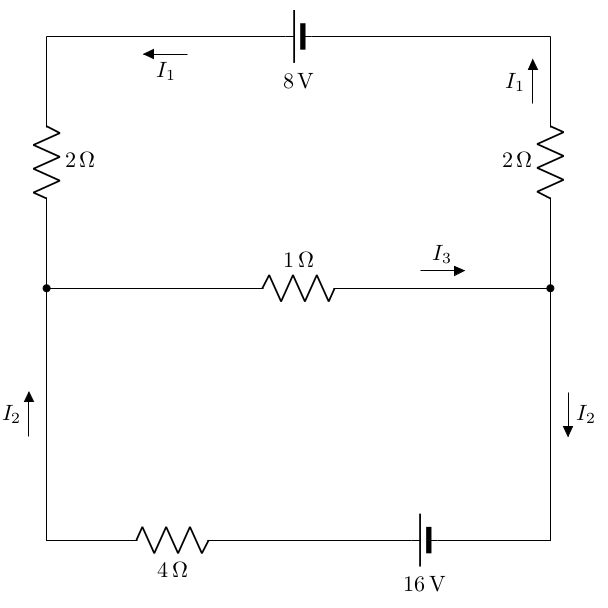
\includegraphics[scale=0.45]{circuit.png}
\end{minipage}
\begin{minipage}{0.35\textwidth}
\paragraph*{Ohm's Law}
	\begin{itemize}
	\item Voltage drop at a resistor is given by $V = IR$.
	\end{itemize}
\paragraph*{Kirchhorff's Laws}
	\begin{itemize}
	\item Junction: Current flowing into a junction must flow out of it.
	\item Path: Sum of IR terms in any direction around a closed path is equal to the total voltage in the path in that direction.
	\end{itemize}
\end{minipage}

\newpage

\section{Terminology}

\subsection{Linear Equation}
$$
a_1 x_1 + a_2 x_2 + \cdots + a_n x_n = b
$$
where
	\begin{itemize}
	\item $a_1$, $a_2$, $\ldots$, $a_n$ are constants.
	\item $n$ is the number of variables.
	\item $x_1$, $x_2$, $\ldots$, $x_n$ are the variables (unknowns).
	\item $b$ is the right-hand side constant term.
	\end{itemize}
	
\spaceP
	
\subsection{Systems of Linear Equations}

\begin{align*}
	a_{11} x_1 + a_{12} x_2 + \cdots + a_{1n} x_n & = b_1 \\
	a_{21} x_1 + a_{22} x_2 + \cdots + a_{2n} x_n & = b_2 \\
	\vdots \phantom{+ + + } & \\
	a_{m1} x_1 + a_{m2} x_2 + \cdots + a_{mn} x_n & = b_m
\end{align*}

where
	\begin{itemize}
	\item $m$ is the number of linear equations.
	\item $n$ is the number of variables.
	\item $a_{11}$, $\ldots$, $a_{mn}$ are constants.
	\item $b_1$, $b_2$, $\ldots$, $b_m$ are the right-hand side constant terms.
	\item $x_1$, $\ldots$, $x_n$ are the variables (unknowns).
	\end{itemize}
	
\spaceP
	
\subsection{Solution of a System of Linear Equations}

A list $(x_1^*, x_2^*, \ldots , x_n^*)$ is a solution to a system of linear equations if it satisfies each equation of the system.

\spaceP

\noindent\underline{Going back to our previous example} 

\newpage

\section{How do we solve systems of linear equations?}

\subsection{Systems of two linear equations with two variables}

	\begin{align*}
	x_1 + x_2 & = 0 \\
	2 x_1 + x_2 & = 1 .
	\end{align*}

\underline{Method 1} (Isolate)
\vspace*{6cm}

\underline{Method 2} (Operations)
\vspace*{6cm}

\subsection{Gauss-Jordan Elimination}

Based on three \textit{elementary operations} on the equations:
	\begin{itemize}
	\item Interchange two equations in the system.
	\item Replace an equation by a multiple of itself.
	\item Replace an equation by itself plus a multiple of another equation.
	\end{itemize}
	
\noindent Main GOAL: transform our system into
	\begin{align*}
	x + 0 y + 0 z &= \tilde{b}_1 \\
	0x + y + 0 z &= \tilde{b}_2 \\
	0x + 0y + z &= \tilde{b}_3 .
	\end{align*}
	\newpage
	
\begin{example}\label{Example:One}
Find the solution(s) to the following system of linear equations:
	\begin{align*}
	x - y + z & = 0 \\
	2x - 3y + 4z & = -2 \\
	-2x - y + z & = 7.
	\end{align*}
\end{example}

\newpage

\subsection{Augmented Matrix}

More efficient way: transform the system in an \textbf{augmented matrix}.

\begin{minipage}{0.45\textwidth}
\begin{align*}
	a_{11} x_1 + a_{12} x_2 + \cdots + a_{1n} x_n & = b_1 \\
	a_{21} x_1 + a_{22} x_2 + \cdots + a_{2n} x_n & = b_2 \\
	\vdots \phantom{+ + + } & \\
	a_{m1} x_1 + a_{m2} x_2 + \cdots + a_{mn} x_n & = b_m
\end{align*}
\end{minipage}
\begin{minipage}{0.025\textwidth}
{\huge $\Rightarrow$}
\end{minipage}
\begin{minipage}{0.45\textwidth}
\begin{align*}
\begin{bmatrix}
a_{11} & a_{12} & \cdots & a_{1n} & b_1 \\
a_{21} & a_{22} & \cdots & a_{2n} & b_2 \\
\vdots & \vdots & \vdots & \vdots & \vdots \\
a_{m1} & a_{m2} & \cdots & a_{mn} & b_m
\end{bmatrix}
\end{align*}
\end{minipage}

\vspace*{24pt}

\begin{example}
Find the augmented matrix of the system of Example \ref{Example:One}.
\end{example}

\vfill

\subsection{Elementary operations revisited}
Elementary operations on linear equations become elementary operations on the rows of the augmented matrix:
	\begin{itemize}
	\item Interchange two rows.
	\item Replace a row by a multiple of itself.
	\item Replace a row by itself plus a multiple of another row.
	\end{itemize}

\newpage

\begin{example}
Solve the system: 
	\begin{center}
	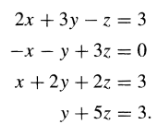
\includegraphics[scale=0.65]{example3-book.png}
	\end{center}		
\end{example}

\newpage

\begin{example}
Solve the system:
	\begin{center}
	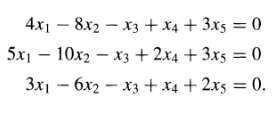
\includegraphics[scale=0.65]{example4-book.png}
	\end{center}
\vspace*{-0.75cm}
\end{example}

\newpage

\section{More Terminology}

\subsection{Reduced row-echelon form}
Transformed augmented matrix after row operations:
	\begin{itemize}
	\item Any rows of zero (called zero rows) appear at the bottom.
	\item The first nonzero entry of a nonzero row is 1 (called a leading 1).
	\item The leading 1 of a nonzero row appears to the right of the leading 1 of any preceding row.
	\item All the other entries of a column containing a leading 1 are zero.
	\end{itemize}

\subsection{Consistent Systems vs Inconsistent Systems}

	\begin{itemize}
	\item \underline{Consistent}: means the system of equations has at least one solution.
		\begin{itemize}
		\item How to recognize that a system is consistent?
		
		(1) \hfill (2) \hfill \phantom{2}
		\vspace*{2cm}
		\end{itemize}
	\item \underline{Inconsistent}: means the system of equations has no solution.
		\begin{itemize}
		\item How to recognize that a system is inconsistent?
		
		(1) 
		\vspace*{2cm}
		\end{itemize}
	\end{itemize}
	
\subsection{Homogeneous System}
\begin{align*}
a_{11} x_1 + a_{12} x_2 + \cdots + a_{1n} x_n & = 0 \\
a_{21} x_1 + a_{22} x_2 + \cdots + a_{2n} x_n & = 0 \\
\cdots \phantom{222222222} & \\
a_{m1} x_1 + a_{m2} x_2 + \cdots + a_{mn} x_n & = 0 
\end{align*}

\begin{itemize}
\item \underline{Trivial solution}: $x_1 = x_2 = \cdots = x_n = 0$.
\end{itemize}

\begin{theorem}
A homogeneous system of $m$ linear equations in $n$ variables
	\begin{itemize}
	\item has infinitely many solutions if $m < n$.
	\item has only the trivial solution if $m= n$.
	\end{itemize}
\end{theorem}

In the other case, when $m > n$, we have to do more work. To be more precised, we still have to find the RREF of the augmented matrix of the associated system and conclude from the RREF if the system has solutions or not.

\newpage

\section{Gaussian Elimination}

\underline{Goal}. Transform the augmented matrix into an new augmented matrix with the following properties:
	\begin{itemize}
	\item any zero rows appear at the bottom.
	\item The first nonzero entry of a nonzero row is $1$.
	\item The leading $1$ of a nonzero row appears to the right of the leading 1 of any preceding row.
	\end{itemize}
	
	\vspace*{16pt}
	
	\begin{example}
	Determine the values of $a$, $b$, and $c$ so that the system
		\begin{align*}
		x - y + 2z &= a \\
		2x + y - z &= b \\
		x + 2y - 3z &= c
		\end{align*}
	has solutions.
	\end{example}

\end{document}